\documentclass[12pt, titlepage]{article}

\usepackage{cite}
\usepackage{booktabs}
\usepackage{tabularx}
\usepackage{hyperref}
\usepackage{amssymb}
\usepackage{amstext}
\usepackage{amsthm}
\usepackage{amsmath}
\usepackage{enumerate}
\usepackage{fancyhdr}
\usepackage[margin=1in]{geometry}
\usepackage{graphicx}
\usepackage{extarrows}
\usepackage{setspace}
\usepackage{adjustbox}


\hypersetup{
    colorlinks,
    citecolor=black,
    filecolor=black,
    linkcolor=red,
    urlcolor=blue
}
% \usepackage[round]{natbib}


% Different Coloured Text and Strikethrough
\usepackage{xcolor}
\usepackage{ulem}

\newcounter{acnum}
\newcommand{\actheacnum}{AC\theacnum}
% \newcommand{\acref}[1]{AC#1}
\newcommand{\acref}[1]{AC\ref{#1}}

\newcounter{ucnum}
\newcommand{\uctheucnum}{UC\theucnum}
\newcommand{\uref}[1]{UC}

\newcounter{mnum}
\newcommand{\mthemnum}{M\themnum}
% \newcommand{\mref}[1]{M#1}
\newcommand{\mref}[1]{M\ref{#1}}


\title{SE 3XA3: Module Guide\\Save The Date}

\author{
        Karuka Khurana (khurak1)\\
        Utsharga Rozario (rozariou)\\
        Samarth Kumar (kumars38)\\
        Dhruv Cheemakurti (cheemakd)\\
}

\date{\today}

\begin{document}

\maketitle

\pagenumbering{roman}
\tableofcontents
\listoftables
\listoffigures

\newpage
\begin{table}[htbp]
    \caption{Revision History} \label{RevisionHistory}
    \begin{tabularx}{\textwidth}{llX}
        \toprule
            \textbf{Date} & \textbf{Developer(s)} & \textbf{Change}\\
        \midrule
            March 15, 2021 & Karuka Khurana & Copy template \& completed introductory section\\\\
            March 16, 2021 & Karuka Khurana & Completed section 5.\\\\
            March 18, 2021 & Karuka Khurana & Completed section 7, 8.\\\\
	 March 18, 2021 & Utsharga Rozario & Completed section 7 Diagram.\\\\
            March 18, 2021 & Dhruv Cheemakurti & Completed section 2, 3, 4, 6.\\\\
        \bottomrule
    \end{tabularx}
\end{table}

\newpage

\pagenumbering{arabic}
\section{Introduction}
\subsection{Overview}
Save The Date is a re-development of an open-source Notion application using React and the Python programming language. Our project aims to further enhance the user experience by adding an additional feature to scrape an uploaded PDF document of a course outline and visualize outstanding dates that are important for students to keep in mind. We hope to promote organization and time management by efficiently displaying important deadlines rather than student’s having to scroll through multiple syllabuses. On top of the original implementation, we will include a PDF upload feature, an option to provide a page range and the option to begin scraping the document. Once this is complete, a dashboard will be created that includes all important dates and deadlines. 

\subsection{Context}
A Software Requirements Specification (SRS) document was created which outlined functional and non-functional requirements this project must fulfill. The purpose of this document is to give a high-level description of the structure of the system which is broken down into modules. Using a unified modelling language (UML) approach, this document will describe the system architecture. Decomposing code into modules will allow for a better understanding of how different aspects of the program communicate with each other to solve a problem. This document has the following sections:

\begin{itemize}
    \item Section 2 outlines any anticipated and unlikely changes
    \item Second 3 outlines the overview of the module hierarchy 
    \item Section 4 outlines the connections between requirements and design 
    \item Section 5 includes the module decomposition 
    \item Section 6 includes two traceability matrices, one for connections between SRS and modules and the another for connections between anticipated changes and modules.
    \item Section 7 includes a hierarchical diagram to visualize the relationship among the modules
\end{itemize}

\subsection{Design Principle}
Modular decomposition is beneficial for many different reasons. Decomposing larger modules into smaller ones ensures reusability, readability, and structure and allows for easy traceability when debugging. In this project, decomposition of the modules is based off of the principle of information hiding (Parnas, 1972). Each of the modules will hide a secret that can easily be changed. \\

Our design follows the rules layed out by (Parnas, 1972), as follows:
\begin{itemize}
\item System details that are likely to change independently should be the
  secrets of separate modules.
\item Each data structure is used in only one module.
\item Any other program that requires information stored in a module's data
  structures must obtain it by calling access programs belonging to that module.
\end{itemize}

\section{Anticipated and Unlikely Changes} 
This sections lists possible changes for the application SaveTheDate. The changes that may occur for the development of an application can be categorized into anticipated and unlikely changes. Anticipated changes are planned or foreseeable whereas unlikely changes are those that were not planned at all. We describe the two categories below.

\subsection{Anticipated Changes} 
\begin{description}

\item[\refstepcounter{acnum} \actheacnum \label{ac1}:]The type of the output of PDFScraper module might change
\item[\refstepcounter{acnum} \actheacnum \label{ac2}:] The format of input data
\item[\refstepcounter{acnum} \actheacnum \label{ac3}:] The PDFScraper module might change as more functionality is added.

\item[\refstepcounter{acnum} \actheacnum \label{ac4}:]The functionality loadPDF module might change as more features will be added. 

\end{description}

\subsection{Unlikely Changes}
\begin{description}
\item[\refstepcounter{ucnum} \uctheucnum \label{uc1}:] There will be a source of input data external to software
\item[\refstepcounter{ucnum} \uctheucnum \label{uc2}:] The system interfacing with background application 
\item[\refstepcounter{ucnum} \uctheucnum \label{uc3}:] Input/output devices
\item[\refstepcounter{ucnum} \uctheucnum \label{uc4}:] The data structures of PDFScraper module output. 
\end{description}

\section{Module Hierarchy} 

\subsection{PDF Scraping subsystem}
\begin{description}
\item[\refstepcounter{mnum} \mthemnum \label{M18}] PDFScraper Module 
\item[\refstepcounter{mnum} \mthemnum \label{M16}] ScrapePDFUser module
\item[\refstepcounter{mnum} \mthemnum \label{M15}] loadPDF module
\item[\refstepcounter{mnum} \mthemnum \label{M17}] image module

\end{description}

\subsection{Table generation subsystem}
\begin{description}
\item[\refstepcounter{mnum} \mthemnum \label{M6}] editableTable module
\item[\refstepcounter{mnum} \mthemnum \label{M7}] Table module
\item[\refstepcounter{mnum} \mthemnum \label{M8}] Cell module
\item[\refstepcounter{mnum} \mthemnum \label{M9}] Text module
\item[\refstepcounter{mnum} \mthemnum \label{M10}] Color module
\item[\refstepcounter{mnum} \mthemnum \label{M11}] Header module
\item[\refstepcounter{mnum} \mthemnum \label{M12}] Relationship module
\item[\refstepcounter{mnum} \mthemnum \label{M13}] util’s module

\end{description}

\subsection{Page generation subsystem}
\begin{description}
\item[\refstepcounter{mnum} \mthemnum \label{M15}] button module
\item[\refstepcounter{mnum} \mthemnum \label{M15}] selectMenu module
\item[\refstepcounter{mnum} \mthemnum \label{M15}] editablePage module
\item[\refstepcounter{mnum} \mthemnum \label{M15}] editableBlock module
\item[\refstepcounter{mnum} \mthemnum \label{M15}] Uid module
\item[\refstepcounter{mnum} \mthemnum \label{M15}] CaretHelpers module

\end{description}
\section{Connection Between Requirements and Design} 
The system design is meant to fulfill all the requirements that were outlined in the SRS. In this stage, the system is decomposed into modules and Table 3 lists the connection between requirements and modules.


\section{Module Decomposition}
The \textbf{Secrets} field in a module decomposition is a brief statement of the design decision hidden by the module. The \textbf{Services} field specifies what the module will do without documenting how to do it. For each module, a suggestion for the implementing software is given under the \textbf{Implemented By} title. If the entry is \textbf{OS}, this means that the module is provided by the operating system or by standard programming language libraries. 

\subsection{Hardware Hiding Modules }
\begin{description}
\item[Secrets:]The data structure and algorithm used to implement the virtual
  hardware.
\item[Services:]Serves as a virtual hardware used by the rest of the
  system. This module provides the interface between the hardware and the
  software. So, the system can use it to display outputs or to accept inputs.
\item[Implemented By:] OS
\end{description}

\subsection{Behaviour-Hiding Module}

\subsubsection{Table Module (M6)}

\begin{description}
\item[Secrets:] Format and structure of the Notion Table
\item[Services:] Renders a table within a Notion page
\item[Implemented By:] Table.js
\end{description}

\subsubsection{Relationship Module (M9)}

\begin{description}
\item[Secrets:] Format and structure of the relationship in a cell of a table.
\item[Services:] Renders a relationship within a table on a Notion page.
\item[Implemented By:] Relationship.js
\end{description}

\subsubsection{Text Module (M10)}

\begin{description} 
\item[Secrets:] Format and structure of the text within in a cell of a table.
\item[Services:] Returns a colour as a string within a table on a Notion page.
\item[Implemented By:] Text.js
\end{description}

\subsubsection{Colors Module (M11)}

\begin{description}
\item[Secrets:] Format and structure of colors within in a cell of a table.
\item[Services:] Renders a color relationship within a table on a Notion page.
\item[Implemented By:] colors.js
\end{description}

\subsubsection{uid Module (M12)}

\begin{description} 
\item[Secrets:] Format and structure of uid generated for EditablePage and EditableBlock.
\item[Services:] Renders a uid and outputs a string to other functions.
\item[Implemented By:] uid.js
\end{description}

\subsubsection{caretHelpers Module (M13)}

\begin{description}
\item[Secrets:] Format and Structure of determining coordinates for EditableBlock module. 
\item[Services:] Retrieves and sets the coordinates.
\item[Implemented By:] caretHelpers.js
\end{description}

\subsubsection{utils Module (M14)}

\begin{description}
\item[Secrets:] Format and Structure of determining IDs and random colours.
\item[Services:] Generates a string output for a short ID and a random colour.
\item[Implemented By:] utils.js
\end{description}

\subsection{Software Decision Module}

\subsubsection{editablePage Module (M1)}

\begin{description}
\item[Secrets:] Format and Structure of a single Notion page.
\item[Services:] Represents the functions that can be executed on a Notion page which includes editing, adding, and deleting.
\item[Implemented By:] editablePage.js
\end{description}

\subsubsection{editableBlock Module (M2)}

\begin{description}
\item[Secrets:] Format and Structure of a block on a single Notion page.
\item[Services:] Represents the functions that can be executed within a block on a Notion page which includes editing, adding, and deleting.
\item[Implemented By:] editableBlock.js
\end{description}

\subsubsection{selectMenu Module (M3)}

\begin{description}
\item[Secrets:] Format and Structure of a menu bar on a single Notion page.
\item[Services:] Represents the functions that can be executed within a menu on a Notion page which includes selecting.
\item[Implemented By:] selectMenue.js
\end{description}

\subsubsection{button Module (M4)}

\begin{description}
\item[Secrets:] Format and Structure of a button on menu bar on a single Notion page.
\item[Services:] Represents the functions that can be executed on a block within a Notion page.
\item[Implemented By:] 
\end{description}

\subsubsection{editableTable Module (M5)}

\begin{description}
\item[Secrets:] Format and Structure of a table on a single Notion page.
\item[Services:] Represents the functions that can be executed within a menu on a Notion page which includes adding, editing, deleting.
\item[Implemented By:] editableTable.js
\end{description}

\subsubsection{Header Module (M7)}

\begin{description}
\item[Secrets:] Format and Structure of a header of a table on a single Notion page.
\item[Services:] Represents the functions that can be executed within a menu on a Notion page which includes selecting.
\item[Implemented By:] Header.js
\end{description}

\subsubsection{Cell Module (M8)}

\begin{description}
\item[Secrets:] Format and Structure of a cell of a table on a single Notion page.
\item[Services:] Represents the functions that can be executed within a menu on a Notion page which includes adding, editing, deleting.
\item[Implemented By:] Cell.js
\end{description}

\subsubsection{loadPDF Module (M15)}

\begin{description}
\item[Secrets:] Accepts the uploaded PDF file.
\item[Services:] Runs through the PDF file to load it in order to scrape the document.
\item[Implemented By:] loadPDF.js
\end{description}

\subsubsection{scrapePDFUser Module (M16)}

\begin{description}
\item[Secrets:] Format and Structure of a pop-up window.
\item[Services:] Allows a user to add a course name and select a PDF file from the pop-up window.
\item[Implemented By:] scrapePDFUser.js
\end{description}

\subsubsection{image Module (M17)}

\begin{description}
\item[Secrets:] Format and Structure of an image on a Notion page.
\item[Services:] Represents the functions that can be executed on an image on a Notion page which includes adding the image and rendering it.
\item[Implemented By:] image.js
\end{description}

\subsubsection{PDFScraper Module (M18)}

\begin{description}
\item[Secrets:] Algorithm to scrape a PDF document.
\item[Services:] Handles obtaining important dates and task information from the uploaded PDF file.
\item[Implemented By:] scraper.py
\end{description}

\section{Traceability Matrix}
This sections shows two traceability matrices: one between modules and requirements, and another between modules and anticipated changes.  
\begin{table}[htbp]
\centering
\begin{tabular}{p{0.2\textwidth} p{0.6\textwidth}}
\toprule
\textbf{Req} & \textbf{Modules}\\
\midrule
FR1 & 4\\
FR2 & 15\\
FR3 & 18\\
FR4 & 6, 8, 10\\
FR5 & 6 \\
FR6 & 6 \\
FR7 & 5 \\
FR8 & 1 \\
FR9 & 15 \\
FR10 & 15 \\
FR11 & 27 \\
FR12 & 4 \\
LF1 & 1 \\
LF2 & 1 \\
UH1 & 4\\
UH2 & 3,4\\
UH3 & 1\\
PE1 & 16 \\
PE2 & 16 \\
PE3 & 16 \\
PE4 & 6 \\
PE5 & N/A\\


\bottomrule
\end{tabular}
\caption{Trace Between Requirements and Modules}
\label{TblACT}
\end{table}





\begin{table}[htbp]
\centering
\begin{tabular}{p{0.2\textwidth} p{0.6\textwidth}}
\toprule
\textbf{AC} & \textbf{Modules}\\
\midrule
\acref{ac1} & 18\\
\acref{ac2} & 15\\
\acref{ac3} & N/A\\
\acref{ac4} & 15\\

\bottomrule
\end{tabular}
\caption{Trace Between Anticipated Changes and Modules}
\label{TblACT}
\end{table}









\section{Use Hierarchy Between Modules}
Figure ? visualizes the use relation between the modules. It can be seen that the graph is a directed acyclic graph (DAG). Each level of the hierarchy offers a testable and usable subset of the system, and modules in the higher level of the hierarchy are essentially simpler because they use modules from the lower levels. 

\begin{figure}[htbp]
\centering
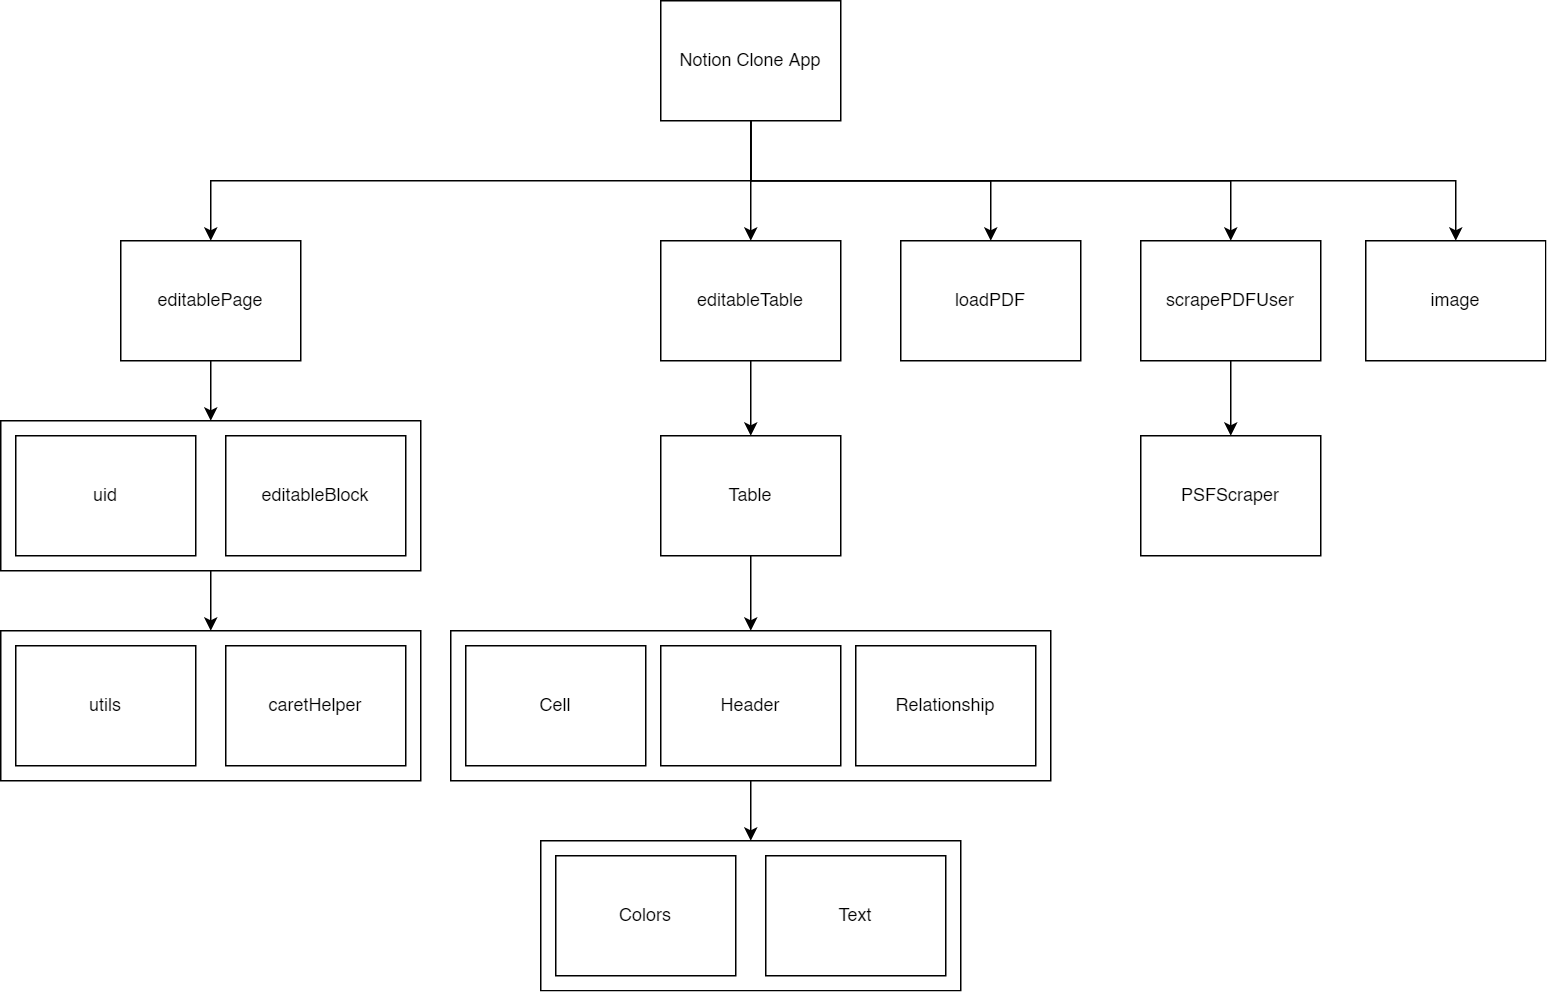
\includegraphics[width=\textwidth]{MG_Hierarchy.png}
\caption{Use Hierarchy Among Modules}
\label{FigUH}
\end{figure}

\section{Schedule}

Implementation dates of the modules along with the team members responsible are available in the Gantt chart.\\

Gantt Chart: \url{https://gitlab.cas.mcmaster.ca/se3xa3_l03_g17/se3xa3_l03_g17/-/blob/main/ProjectSchedule/3XA3_L03_G17_GanttChart.pdf}

\section{References}

\bibliographystyle {plainnat}
\bibliography {MG}

David L. Panas. On the criteria to be used in decomposing systems into modules. Comm.ACM, 15(2):1053 1058, December 1972\\

D.L. Parnas, P.C. Clement, and D. M. Weiss, The modular structure of complex systems. In International Conference on Software Engineering, pages 408-419, 1984.

\end{document}